\documentclass[aspectratio=169, pdf, 8pt, unicode]{beamer}
\usepackage[american,russian]{babel}
\usepackage[default]{sourcesanspro}
\usepackage{float}
\usepackage{graphicx}
\usepackage{pgfplotstable}
\usepackage{caption}
\usepackage{amsmath}
\usepackage{amssymb}
\usepackage{setspace}
\usepackage{fancyvrb}
\usepackage[outputdir=aux]{minted}

\DeclareCaptionLabelFormat{gostfigure}{Рисунок #2}
\captionsetup[table]{labelsep=endash,justification=justified,singlelinecheck=false,font=normalsize,skip=0pt} 
\captionsetup[figure]{labelformat=gostfigure,labelsep=endash,justification=centering,singlelinecheck=false,font=normalsize} 
\pgfplotsset{compat=1.9}

\mode<presentation> {
\usetheme{Madrid}
}

\setbeamerfont{institute}{size=\normalsize}
\setbeamertemplate{itemize/enumerate body begin}{\large}
\setbeamertemplate{itemize/enumerate subbody begin}{\tiny}

\title[Теория и практика многопоточного программирования]{Теория и практика многопоточного программирования\\ \vspace{0.5cm}Семинар 4}

\author{Неганов Алексей}

\institute[МФТИ]{
    Московский физико-технический институт (национальный исследовательский университет)\\
    Кафедра теоретической и прикладной информатики\\
}

\date{Москва 2020}

\setbeamertemplate{caption}[numbered]

\begin{document}

\begin{frame}
\titlepage
\end{frame}

\begin{frame}[fragile]
\frametitle{RMW-операции: ABA}
LL/SC:
\begin{figure}[H]
\centering
%\begin{BVerbatim}
\begin{minipage}{0.8\textwidth}
\begin{minted}{C}
word LL(word *ptr) {
   return *ptr; // and set cache line status bit simultaneously
}

bool SC(word *ptr, word newval) {
   if ( /* cache line bit is set */ ) {
      *ptr = newval;
      return true ;
   }
   else
      return false ;
}

bool CAS(word *ptr, word oldval, word newval) {
   if (LL(ptr) == oldval)
      return SC(ptr, newval);
   return false ;
}
\end{minted}
\end{minipage}
%\end{BVerbatim}
\end{figure}
\end{frame}

\begin{frame}[fragile]
\frametitle{Барьеры памяти}
\hspace{0.05\textwidth}
\begin{minipage}{0.2\textwidth}
\begin{figure}[H]
\centering
\begin{BVerbatim}
int a = 0;
int b = 0;

void foo(void) {
      a = 1;
      b = 1;
}

void bar(void) {
      while(b == 0);
      assert(a == 1);
}
\end{BVerbatim}
\end{figure}
\end{minipage}
\begin{minipage}{0.7\textwidth}
\begin{figure}[H]
      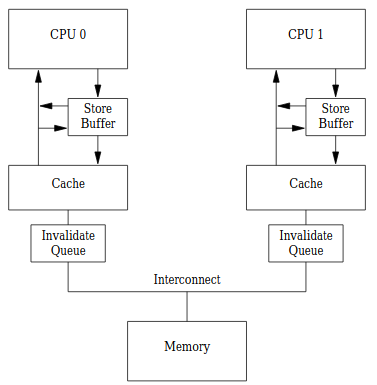
\includegraphics[width=0.5\textwidth]{fig/store_buffers.png}
\end{figure}
\end{minipage}
\end{frame}

\begin{frame}[fragile]
\frametitle{Барьеры памяти}
\hspace{0.05\textwidth}
\begin{minipage}{0.2\textwidth}
\begin{figure}[H]
\centering
\begin{BVerbatim}
int a = 0;
int b = 0;

void foo(void) {
      a = 1;
      smp_wmb();
      b = 1;
}

void bar(void) {
      while(b == 0);
      smp_rmb();
      assert(a == 1);
}
\end{BVerbatim}
\end{figure}
\end{minipage}
\begin{minipage}{0.7\textwidth}
\begin{figure}[H]
      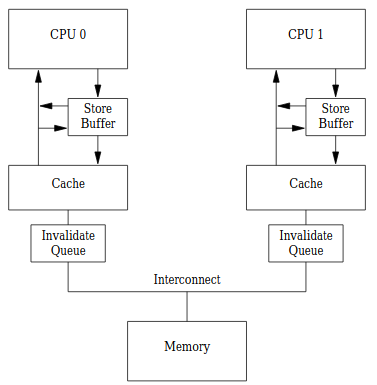
\includegraphics[width=0.5\textwidth]{fig/store_buffers.png}
\end{figure}
\end{minipage}
\end{frame}

\begin{frame}[fragile]
\frametitle{Модели памяти: relaxed}
\begin{figure}[H]
\begin{BVerbatim}
// 'memory_order_relaxed' argument is omitted for brevity
atomic_t x, y;
x.store(0);
y.store(0);

y.store(20);      if (x.load() == 10) {          if (y.load() == 10)
x.store(10);        assert (y.load() == 20)        assert (x.load() == 10);
                    y.store (10);
                  }
\end{BVerbatim}
\end{figure}
Load/store операции могут переупорядочиваться, может сработать и тот, и другой \texttt{assert}.
\begin{figure}[H]
\begin{BVerbatim}
x.store(1);      y = x.load();
y.store(2);      z = x.load();
                 assert(y <= z);
\end{BVerbatim}
\end{figure}
Гарантия -- \texttt{assert} не может сработать.
\end{frame}

\begin{frame}[fragile]
\frametitle{Модели памяти: sequentially consistent}
\begin{figure}[H]
\begin{BVerbatim}
atomic_t x, y;
x.store(0);
y.store(0);

y.store(20);      if (x.load() == 10) {          if (y.load() == 10)
x.store(10);        assert (y.load() == 20)        assert (x.load() == 10);
                    y.store (10);
                  }
\end{BVerbatim}
\end{figure}
Load/store операции могут выполняться лишь в том порядке, что и в коде, ни один \texttt{assert} выполниться не может.
\begin{figure}[H]
\begin{BVerbatim}
atomic_t x;
x.load(0);
int y = 0;

y = 1            if (x.load() == 2)
x.store(2);        assert (y == 1)
\end{BVerbatim}
\end{figure}
Запись в $y$ в коде происходит до записи в $x$, следовательно, \texttt{assert} выполниться не может.
\end{frame}

\begin{frame}[fragile]
\frametitle{Модели памяти: acquire/release}
\begin{figure}[H]
\begin{BVerbatim}
load memory, register ;
membar #LoadLoad | #LoadStore ; // acquire barrier

...

membar #LoadStore | #StoreStore ; // release barrier
store regiser, memory
\end{BVerbatim}
\end{figure}
\end{frame}

\begin{frame}[fragile]
\frametitle{Модели памяти: acquire/release}
\begin{figure}[H]
\begin{BVerbatim}
#define A memory_order_acquire
#define R memory_order_release

// thread 1                                   // thread 2
y.store(20, R);                               x.store(10, R);

// thread 3                                   // thread 4
assert(y.load(A) == 20 && x.load(A) == 0);    assert(y.load(A) == 0 && x.load(A) == 10); 
\end{BVerbatim}
\end{figure}

В sequential consistency один из \texttt{assert} сработает, в acquire/release --- оба могут пройти.

\begin{figure}[H]
\begin{BVerbatim}
// 'memory_order_XXX' argument is omitted for brevity
atomic_t x, y;
x.store(0);
y.store(0);

y.store(20);      if (x.load() == 10) {          if (y.load() == 10)
x.store(10);        assert (y.load() == 20)        assert (x.load() == 10);
                    y.store (10);
                  }
\end{BVerbatim}
\end{figure}

В acquire/release \texttt{assert} второго потока пройдёт, а третьего --- сработает.

\end{frame}

\begin{frame}[fragile]
\frametitle{Spinlock}
\begin{figure}[H]
\centering
\begin{minipage}{0.8\textwidth}
\begin{minted}{C++}
class spin_lock_TAS
{
    atomic<unsigned int> m_spin ;
public:
    spin_lock(): m_spin(0) {}
    ~spin_lock() { assert( m_spin.load(memory_order_relaxed) == 0);}

    void lock()
    {
        unsigned int expected;
        do { expected = 0; }
        while ( !m_spin.compare_exchange_weak( expected, 1, memory_order_acquire ));
    }
    void unlock()
    {
        m_spin.store( 0, memory_order_release );
    }
};
\end{minted}
\end{minipage}
\end{figure}
\end{frame}

\begin{frame}[fragile]
\frametitle{Spinlock}
\begin{figure}[H]
\centering
\begin{minipage}{0.8\textwidth}
\begin{minted}{C++}
class spin_lock_TTAS
{
    atomic<unsigned int> m_spin ;
public:
    spin_lock(): m_spin(0) {}
    ~spin_lock() { assert( m_spin.load(memory_order_relaxed) == 0);}

    void lock()
    {
        unsigned int expected;
        do {
            while (m_spin.load(memory_order_acquire));
            expected = 0;
        }
        while ( !m_spin.compare_exchange_weak( expected, 1, memory_order_acquire ));
    }
    void unlock()
    {
        m_spin.store( 0, memory_order_release );
    }
};
\end{minted}
\end{minipage}
\end{figure}
\end{frame}

\begin{frame}[fragile]
\frametitle{Spinlock}
\begin{figure}[H]
\centering
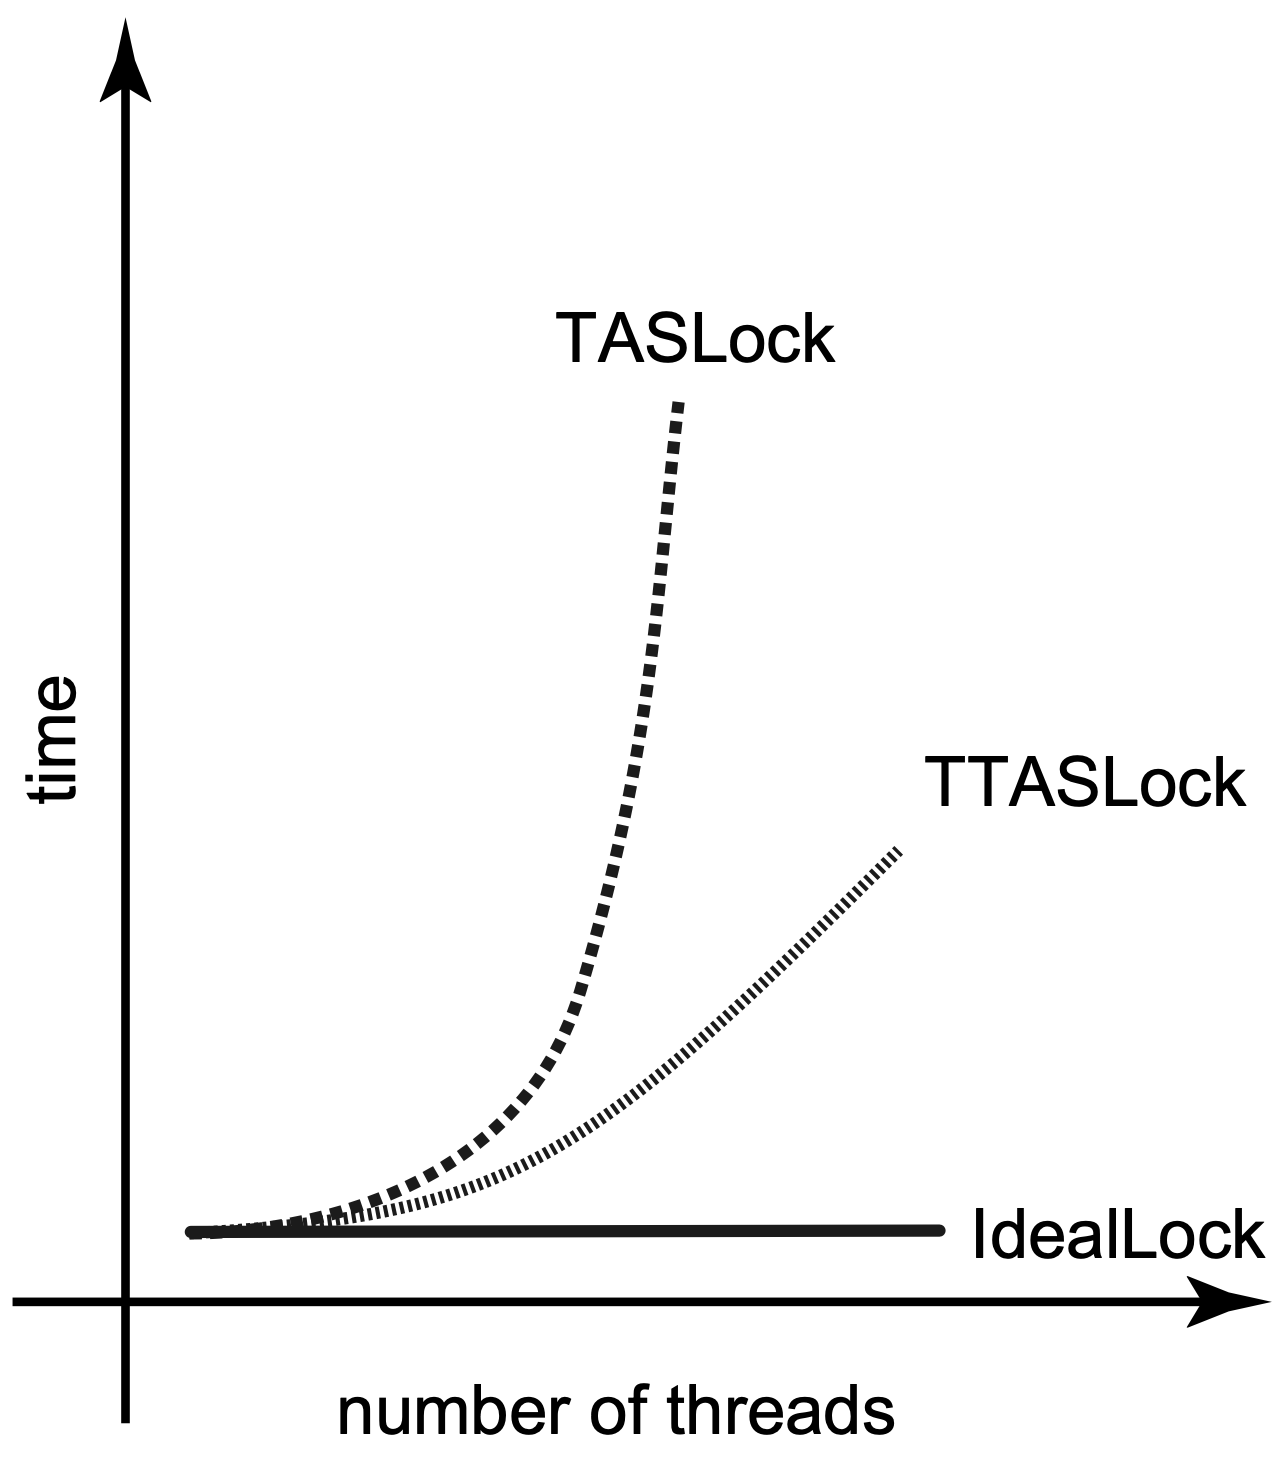
\includegraphics[width=0.4\textwidth]{fig/tas_vs_ttas.png}
\end{figure}
\end{frame}

\begin{frame}[fragile]
\frametitle{Жизненный цикл потока: yield vs sleep}
\begin{figure}[H]
\centering
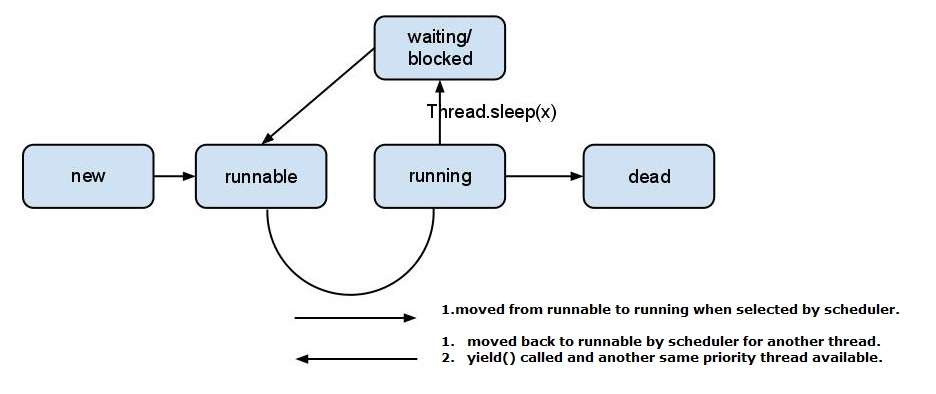
\includegraphics[width=1.0\textwidth]{fig/yield_vs_sleep.jpg}
\end{figure}
\end{frame}

\begin{frame}
\frametitle{Задачи}
\begin{enumerate}
\item \textbf{(Обязательная)} Напишите свои mutex'ы, использующие yield / exponential backoff.
    Сравните производительность TAS lock / TTAS lock / lock with yield / backoff lock.
    Желательно использовать C++11 (и выше), при желании можно GNU С11 и pthreads.
\end{enumerate}

Доклады:
\begin{enumerate}
\item Протоколы MESI, MOESI, MESIF.
\item Барьеры памяти в x86 с примерами на ассемблере. Связь с memory order из C11 / C++11.
\end{enumerate}

\end{frame}

\end{document}
